\documentclass[onecolumn, draftclsnofoot,10pt, compsoc]{IEEEtran}
\usepackage{graphicx}
\usepackage{url}
\usepackage{setspace}
\usepackage{enumitem}
\usepackage{longtable}
\usepackage{listings}

\usepackage{geometry}
\geometry{textheight=9.5in, textwidth=7in}

% 1. Fill in these details
\def \CapstoneTeamName{		}
\def \CapstoneTeamNumber{		6}
\def \GroupMemberOne{			Donghao Lin}
\def \GroupMemberTwo{			Joshua Diedrich}
\def \GroupMemberThree{			Christopher Breniser}
\def \CapstoneProjectName{		Race Car Scanning and Modeling}
\def \CapstoneSponsorCompany{	REHV}
\def \CapstoneSponsorPersonOne{	Kyson Montague}
\def \CapstoneSponsorPersonTwo{	Rodney Stauber}

% 2. Uncomment the appropriate line below so that the document type works
\def \DocType{	
				%Requirements Document
				%Technology Review
				Design Document
				%Progress Report
				}
			
\newcommand{\NameSigPair}[1]{\par
\makebox[2.75in][r]{#1} \hfil 	\makebox[3.25in]{\makebox[2.25in]{\hrulefill} \hfill		\makebox[.75in]{\hrulefill}}
\par\vspace{-12pt} \textit{\tiny\noindent
\makebox[2.75in]{} \hfil		\makebox[3.25in]{\makebox[2.25in][r]{Signature} \hfill	\makebox[.75in][r]{Date}}}}
% 3. If the document is not to be signed, uncomment the RENEWcommand below
%\renewcommand{\NameSigPair}[1]{#1}

%%%%%%%%%%%%%%%%%%%%%%%%%%%%%%%%%%%%%%%
\begin{document}
\begin{titlepage}
    \pagenumbering{gobble}
    \begin{singlespace}
    	
\includegraphics[height=4cm]{coe_v_spot1}
        \hfill 
        % 4. If you have a logo, use this includegraphics command to put it on the coversheet.
        %\includegraphics[height=4cm]{CompanyLogo}   
        \par\vspace{.2in}
        \centering
        \scshape{
            \huge CS Capstone \DocType \par
            {\large\today}\par
            \vspace{.5in}
            \textbf{\Huge\CapstoneProjectName}\par
            \vfill
            {\large Prepared for}\par
            \Huge \CapstoneSponsorCompany\par
            \vspace{5pt}
            {\Large\NameSigPair{\CapstoneSponsorPersonOne}\par}
            {\Large\NameSigPair{\CapstoneSponsorPersonTwo}\par}
            {\large Prepared by }\par
            Group\CapstoneTeamNumber\par
            % 5. comment out the line below this one if you do not wish to name your team
            \CapstoneTeamName\par 
            \vspace{5pt}
            {\Large
                \NameSigPair{\GroupMemberOne}\par
                \NameSigPair{\GroupMemberTwo}\par
                \NameSigPair{\GroupMemberThree}\par
            }
            \vspace{20pt}
        }
        \begin{abstract}
        % 6. Fill in your abstract    
        	Indie Lights racing is a dangerous sport and as such, needs safety standards to mitigate that danger whenever possible. We will be working with Compliance software development company REHV to develop a process of scanning vehicles wheels prior to participating in a race to gather useful data faster than traditional methods. The proposed solution reduce the number of hand measurements that must occur to speed up the inspection process. 
        \end{abstract}     
    \end{singlespace}
\end{titlepage}
\newpage
\pagenumbering{arabic}
\tableofcontents
% 7. uncomment this (if applicable). Consider adding a page break.
%\listoffigures
%\listoftables
\clearpage

% 8. now you write!
\section{Document Overview}
\subsection{Scope}
The project described in this document will be used by the REHV development team as a base for testing and creating a system to measure Indy Lights series race car wheels to check for compliance prior to a race. We will be assisting REHV in creating a race car wheel measuring software by developing the back-end to that software. The goal is to take images in from up to 4 stereo cameras and produces precise measurements about the vehicle wheels. This will be done over the coarse of about 6 months of work. 

\subsection{Purpose}
The purpose of this document is to layout the base for our approach in satisfying out requirements document. We will be referring to this document throughout our development process. This document will also serve the purpose of describing our outline to our client and appropriate parties. 

\subsection{Intended Audience}
This document has been compiled for the REHV development team and any of their partnering affiliates. This is also created for the “Race Car Scanning and Modeling project” team to reference as the progress of this software moves forward.

\subsection{Definitions} 
\begin{longtable}{|p{1.5cm}|p{15cm}|}

\caption{A sample long table.} \label{tab:long} \\

\hline \multicolumn{1}{|c|}{\textbf{Term}} & \multicolumn{1}{c|}{\textbf{Definition}} \hline
\endfirsthead

REHV & An organization that develops Indey Lights race car related software. They are known for there TechWorks system and introducing digital measurement tracking during pre-race inspections. 
\hline
CARS & Camera Assisted Race-car Scanning
\hline
Chassis & The central body of the car, including the driver's compartment. Also referred to as the "tub."
\hline
Camber & Degree to which front tires lean in toward the car (from the top of the tire) and the left-side tires lean out. A useful tool to gain grip in corners by maximizing the amount of tire-to-track contact
\hline
Toe & Refers to the alignment of the front and rear tires. If tires point inward, the condition is called "toe-in." If tires point outward, the condition is called "toe-out." Correct toe settings are essential in order to maximize grip.
\hline
Wheelbase & The distance between the centers of the front and rear wheels. 
\hline
OpenCV & A library of programming functions mainly aimed at real-time computer vision.
\hline
Contour & An outline of an object that OpenCV can detect and distinguish from surrounding pixels.  
\hline
ZED Stereo Camera & A device comprised of two separate cameras a known distance away from another. These cameras allow the capture of depth information when used in combination with the ZED SDK. 
\hline
ZED SDK & A library of programming functions to take advantage of the ZED Stereo Cameras ability to capture 3D images and process depth maps.
\hline
SDK & Software Development Kit
\hline

\end{longtable}

\section{Design Description} 
\subsection{Overview}
The following section will specify the design that will be used to locate and measure the objects on our wheel mounts. This involves using the Open-CV library, and it's embedded algorithms to find each shape in our image that is necessary to acquire our needed measurements.

\subsection{System Setup}
Our software will require having a computer with a few main components. First is the ZED SDK. This will allow us to use the libraries provided by ZED to capture depth maps. This SDK requires the use of CUDA 10.1, provided by Nvidia to work properly. This will also require that we have a graphics card with Nvidia architecture. Finally, we will need to use the libraries provided by OpenCV. To incorporate all of these libraries we will be building a visual studios project with cmake. 

\subsection{Image Capturing System}
We will have two cameras for our demo setup each pointing at a different image. We will be using one computer with two ZED cameras connected via USB3.0. The ZED SDK provides a setup routine to initialize these cameras.  This just involves creating ZED objects, and using the grab function to take an image.  These images can be stored in image objects, which also come with the SDK.

\subsection{Image Processing}
Once taken from our stereo cameras, the images will be processed using computer vision.  The goal is to receive an image from our camera, and locate five identifiable squares at the center of our fiducials.
We will begin our image processing by running through our entire image and locating every contour that resembles a square.  This involves using the properties of squares, and eliminating contours that dont match those properties.
\subsubsection{Noise Reduction}
Noise reduction is done simply by downscaling our image, and subsequently upscaling it.  This should help make our image have more clear edges.  Downscale and upscale are both functions you can find with OpenCV. They are called pyrDown and pyrUp respectively.

\subsubsection{Finding Contours}
Once we finish reducing noise, we need to find contours in our image.  The first step in doing this is applying edge detection to image.  Edge detection scans the image for all the edges.  Since our squares have crisp edges with good contrast behind them, these edges will certainly be found.  Once noise reduction and edge detection have been applied to an image, the result looks something like this.  Below is an image that has been passed into the edge detection function called Canny.
\newline
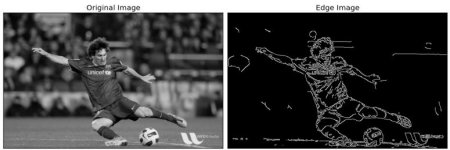
\includegraphics[height=4cm]{Images/canny1.jpg}
\newline
An image like this will make finding contours much more efficient and accurate.  Contour locating can simply be done using the findContours function available in OpenCV.  In  our case we will store all of our contours in a list.
\subsubsection{Checking Vertices}
Once all of the contours are stored in a list in our program, we can safely assume that the five squares we want to find in our fiducials are members of that list.  The key features we can use to find instances of square shapes are the corners.  Squares should all have four corners, and each corner should have an angle very close to 90 degrees.  We can use this to our advantage to weed out contours which do not match this description
\newline
\newline
First we can take a polygonal approximation of each contour.  We can take each contour that we found and approximate a polygon for it.  This approximated polygon can then give us a list of points corresponding to each corner of our shape.  If this list is not equal to exactly four, we can go ahead and throw out that shape.
\newline
\newline
At this point in our square detection we should have a list of all of the shapes in our images which have four corners.  Our final check will be on the angles of these four corners.  Since we will have four coordinate points of each contour corresponding to their corners, we can use some math to find the angle between each set of adjacent edges.  If we have three points p1, p2, and p3,  we can find the effective angle (assuming it is at point p2) with the following using the dot product  formula for two lines.  Once we find the angle, we will check if its cosine is close to 0.  If the angle of every corner of one contour is very close to 0, we can be quite confident that the contour is a square.  Each contour that passes these tests can then be saved in a list of squares.
\subsubsection{Depth Fixing}
Our method for finding all the squares in our image will likely leave us with squares in the background that are unnecessary.  We want to end up with only the five squares located on our fiducial plate.  To minimize these extra squares we can apply tests that help us decide if they are intended. The first test we can make on all of our squares is a depth check.  We know that our wheel will be located no more than 600 millimeters from the lens of our camera. We can ensure our squares are at the right depth by looping through them and taking a depth measurement for each.  If this depth measurement is greater than 600 millimeters, we are safe to remove that square from our list, as it is too far away to be on the fiducial plate.

\subsubsection{Averaging}
Our fiducial (image can be seen in physical setup) is laid out such that each of the four outside squares are equidistant to the center square.  Because of this specific layout, we know that the average pixel value for our surrounding squares should be very close to the pixel measurement we get for the center square.  We can take every combination of size 4 in our image, average the pixel coordinates for them, and check to see that the given average matches another square in our image.  If one of the existing squares is within a few pixels of our average, we have a very confident guess that the currently selected five squares are the ones we want to keep.

\subsection{Measuring Depth and Offset}
Our system needs to find the effective depth for each of the squares found during our image processing. It also needs to find an offset for the center of the wheel.

\subsubsection{Depth Map}
The ZED SDK has a number of tools that will allow us to find the depth of each of our squares.  The way to do this is actually very simple.  There is a function called getDepthMap, which will return a Mat Image object.  This image object has functions that we can use to actually get specific values located on the map.  After we create a depth map and get an image object, we can retrieve the depth at specific values by passing in pixel coordinates.

\subsubsection{Point Cloud}
In addition to the depth map, the ZED SDK has an Image object called a point cloud.  A point cloud maps each point in an image with an x, y, z, and color value.  These x, y, and z values are all returned in millimeters.  The origin for the point cloud starts at the cameras left eye, where the coordinates would be (0,0,0).  By retrieving our x and y values in millimeters from the point cloud, we can obtain an offset for our wheel relative to the camera.


\subsection{IO}
The input for our system is going to be very simple.  There will be a simple run command, which will start the program. The program should output marked up photos of the images, and a list of the final measurements in the console.  Marking up our image can be done simply with functions on OpenCV.  This involves passing in a point to the drawing function called circle, and choosing mark size.

\end{document}